\documentclass{article}
\usepackage[T1]{fontenc}
\usepackage[utf8]{inputenc}
\usepackage{graphicx}
\usepackage{amsmath}
\usepackage[margin=2cm]{geometry}
\sloppy
\begin{document}
\section*{Nabla teaching}
Sintetico: True\par
\subsection*{Learning objectives}
Bounded examples. NIST data are published observations; other examples are synthetic.\par
Evidencias: \par
\subsection*{Assumptions}
Bounded examples. NIST data are published observations; other examples are synthetic.\par
Evidencias: \par
\subsection*{Worked examples}
Bounded examples. NIST data are published observations; other examples are synthetic.\par
Evidencias: \par
\begin{center}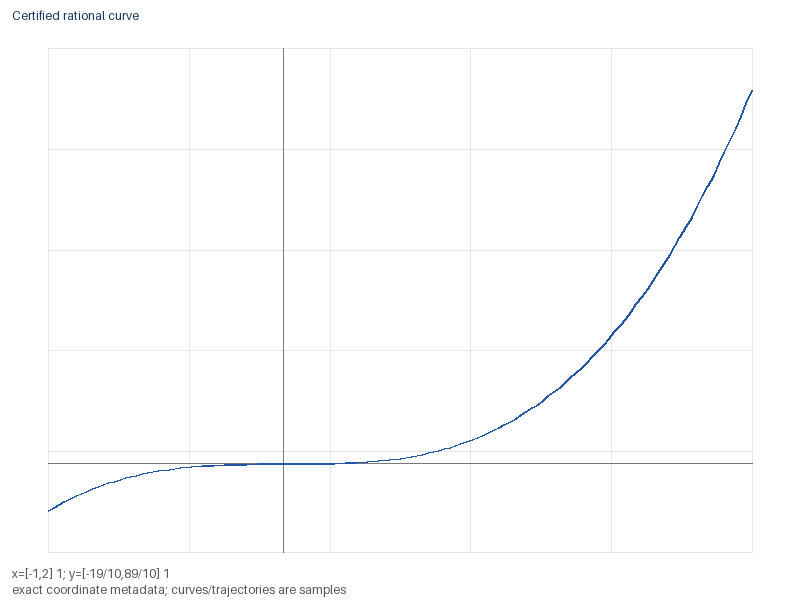
\includegraphics[width=.8\linewidth]{figures/f3261dfff008a68ee41216c84039bf0c63d89bbc2619104b99abfeee2d81cfc2.png}\par
Model-linked rational curve, vertical interpolation tolerance 1/1000; source scene is replayable.\par
\end{center}
\begin{center}
Reproduced computational evidence\par
\begin{tabular}{ll}
Check & Outcome\\ \hline
Published NIST numerical reference & passed\\
Durable agent resume & passed\\
Rational basis holdout & matched\\
Signed delta exchange & passed\\
\end{tabular}
\par Evidencias: 9eed1c8826a38cf24654fee2\allowbreak{}4f84512a9fcfc8d5b56fd7a0\allowbreak{}9114a957dcc6088b, 9c5acec0437fce273798a9f2\allowbreak{}2d1e243c36790ae477a87b6b\allowbreak{}ba72adca5b04ab0e, 6a3ffb90d9449d43e21b68f3\allowbreak{}2af5401aec416639a9d79e73\allowbreak{}feea8249b6f5e834, b63ec06bf5dc75bcd400f970\allowbreak{}97748a1a147898639c3de64b\allowbreak{}42a7642124c39cb3
\end{center}
\subsection*{Exercises}
Bounded examples. NIST data are published observations; other examples are synthetic.\par
Evidencias: \par
\subsection*{Solutions}
Bounded examples. NIST data are published observations; other examples are synthetic.\par
Evidencias: \par
[ref\_9461a7201cac9c1b4e5b5bb0] J. W. Longley (1967). An Appraisal of Least Squares Programs for the Electronic Computer from the Viewpoint of the User. https://github.com/statsmodels/statsmodels\par
Computational checks only; no global novelty, physical validation or independent peer review.
\end{document}
